\chapter{Herramientas software y hardware}\label{sec:Herramienta_software _y _hardware}
\section{Biosignalplux}
Para la adquisición usaremos el kit de investigación de Biosignalplux de 8 canales. Utiliza el software OpenSignals para adquirir y visualizar simultáneamente hasta 8 sensores de EMG. \newline
\begin{figure}[H]
	\center
	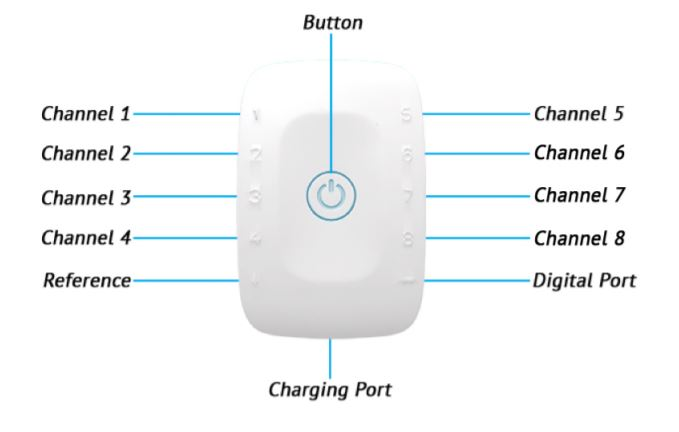
\includegraphics[scale=0.8]{imagenes/Herramientas/Bios.jpg}
	\caption{Hub de Biosignalplux}
	\label{fig:Biosignalplux}
\end{figure}
Con respecto a su utilización simplemente hay que conectar los electrodos para la captación de señales EMG que vienen con el kit Biosignalplux, y conectarlos en cualquiera de los 8 canales de los que disponemos.  Cabe destacar la importancia del puerto de referencia, que colocándolo en una superfice neutra de nuestro cuerpo nos permitirá obtener señales EMG mucho más precisas. \newline 

El hub de Biosignalplux cuenta con conexión Bluethooth, por lo que para captar los datos que nos interesan basta con conectarlo mediante Bluethoot a un ordenador con el software de OpenSignals. Tras la selección del canal ya empezaremos a ver las señales en tiempo real automáticamente, las cuáles podrán ser guardadas para su posterior estudio en este mismo programa. \newline

\begin{figure}[H]
	\center
	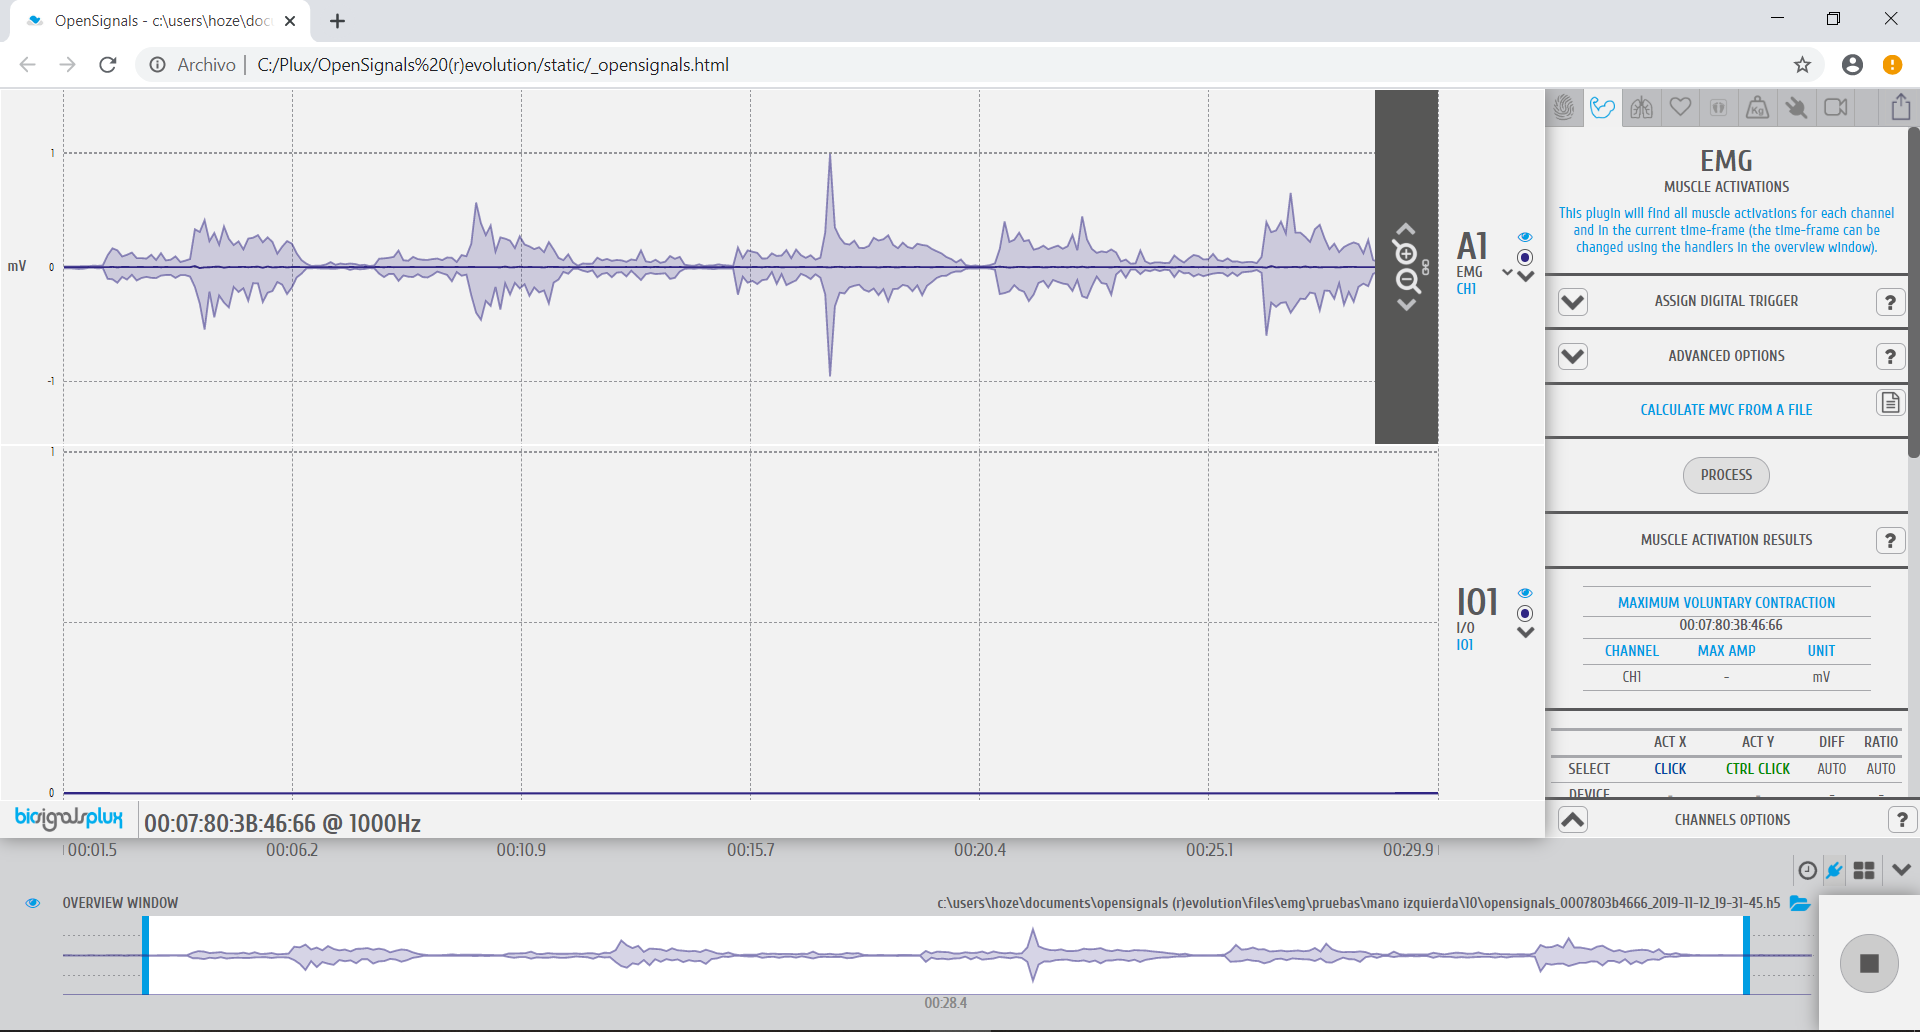
\includegraphics[scale=0.3]{imagenes/Herramientas/OpenSignals.png}
	\caption{Ventana de OpenSignals con una señal EMG}
	\label{fig:OpenSignals}
\end{figure}

 
\section{Matlab}
Es un programa de cálculo numérico el cual cuenta con su propio lenguaje de programación. Permite la comunicación con dispositivos hardware así como la visualización y programación de manera fácil e intuitiva dónde las soluciones se expresan como funciones matemáticas.\newline 

 Como ventaja permite resolver problemas computacionales en un tiempo menor de lo que tardaría un lenguaje escalar no interactivo como C. \newline
\section{FPGAS}
Una \textit{FPGA} (Field Programmable Gate Array) es un dispositivo programable con bloques lógicos cuya interconexión puede ser configurada mediante un lenguaje de descripción para crear circuitos digitales.\newline

Están compuestos internamente por puertas lógicas, cables y biestables; todo ello sin conectar, como una plantilla en blanco. Para su programación requiere la carga de un archivo con la descripción del circuito - o bitstream- que define las uniones entre los biestables y puertas lógicas para crear el circuito que deseemos. 

\begin{figure}[H]
	\center
	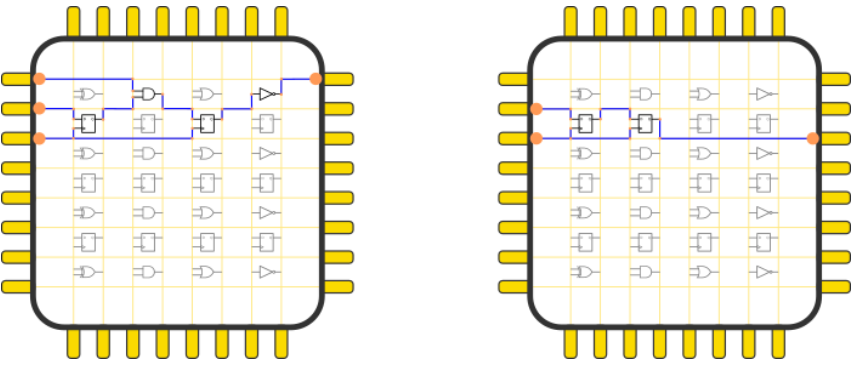
\includegraphics[scale=0.6]{imagenes/Herramientas/FPGA.png}
	\caption{Estructura interna de una FPGA}
	\label{fig:Estructura interna de una FPGA}
\end{figure}

\subsection{FPGAs vs MCU}

Las \textit{FPGA} y los \textit{MCU} (microcontroller unit - microcontrolador) son dos de las herramientas más poderosas disponibles para un ingeniero eléctronico en la actualidad. Es esencial para cualquier persona que trabaje en electrónica digital, como para un profesional en cualquier industria, o incluso un aficionado, obtener una comprensión completa de las herramientas disponibles para ayudar en su trabajo. Esto es especialmente cierto en una industria acelerada, donde las herramientas y tecnologías están sujetas a cambios repentinos y frecuentes.\newline

\begin{figure}[H]
	\center
	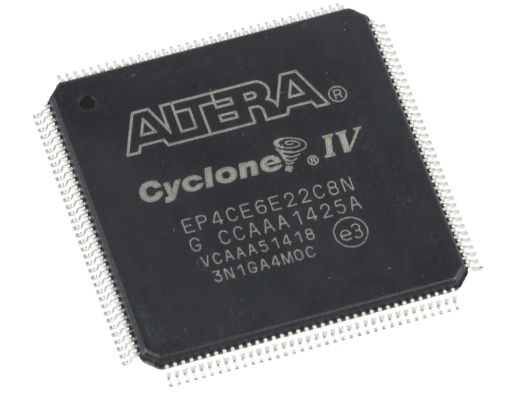
\includegraphics[scale=0.6]{imagenes/Herramientas/FPGA2.png}
	\caption{FPGA EP4CE6E22C8N}
	\label{fig:FPGA EP4CE6E22C8N}
\end{figure}


\begin{figure}[H]
	\center
	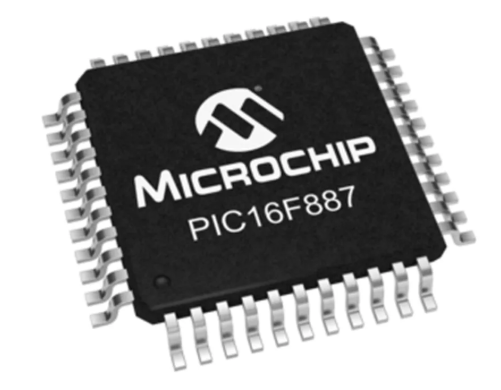
\includegraphics[scale=0.6]{imagenes/Herramientas/MCU.png}
	\caption{MCU PIC16F887}
	\label{fig:MCU PIC16F887}
\end{figure}


Estos dispositivos se usan generalmente en escenarios muy similares; para decirlo de manera muy amplia: los dos permiten introducir unos valores de entrada y obtener los cambios que deseemos en las salidas. De hecho, casi cualquier aplicación que use un microcontrolador podría emplearse en una FPGA para el mismo efecto, y viceversa. Esto no quiere decir que las dos tecnologías sean intercambiables; a veces lo que es muy difícil lograr usar en un dispositivo, podría ser una cuestión simple para el otro.\newline 

La diferencia más importante entre los microcontroladores y las FPGAs es la forma en que procesan las instrucciones. Los primeros  procesan comandos secuencialmente, lo que significa que un micro lee cada línea del programa de una en una, en secuencia. Por el contrario, los FPGA procesan comandos simultáneamente, por lo que las líneas de código se ejecutan a la vez; traduciéndose en un incremento de la velocidad. Además en un microprocesador cada instrucción está asociada a un hardware de manera fija, y el programador no puede usar más instrucciones de las que le ofrece el fabricante. Las FPGAs no tienen nada conectado de manera fija, el usuario es el que determina mediante conexiones el comportamiento del circuito. \newline
Debido a esto las FPGAs generalmente se usan en escenarios que requieren un procesamiento de datos en paralelo de alta velocidad, o un alto grado de personalización, pero pueden resultar engorrosas por su relativa complejidad de configuración. Mientras tanto, los MCU son mucho más fáciles de configurar y usar desde el principio, manejan de manera aceptable los datos en serie de alta velocidad y su producción es más barata. \newline

Sin embargo, el panorama actual de los MCUs está a punto de cambiar debido al estancamiento de la ley de Moore. \ref{sec:Moore}\newpage

\subsubsection{El estancamiento de la ley de Moore}\label{sec:Moore}

La Ley de Moore es la observación empírica realizada el 19 de abril de 1965 por Gordon Moore, cofundador de Intel , en la que postulaba que el número de transistores por unidad de superficie de un microprocesador iba a duplicarse cada 2 años- y por lo tanto la velocidad del procesador o la potencia de procesamiento general-, al menos durante las siguientes dos décadas.\newline


\begin{figure}[H]
	\center
	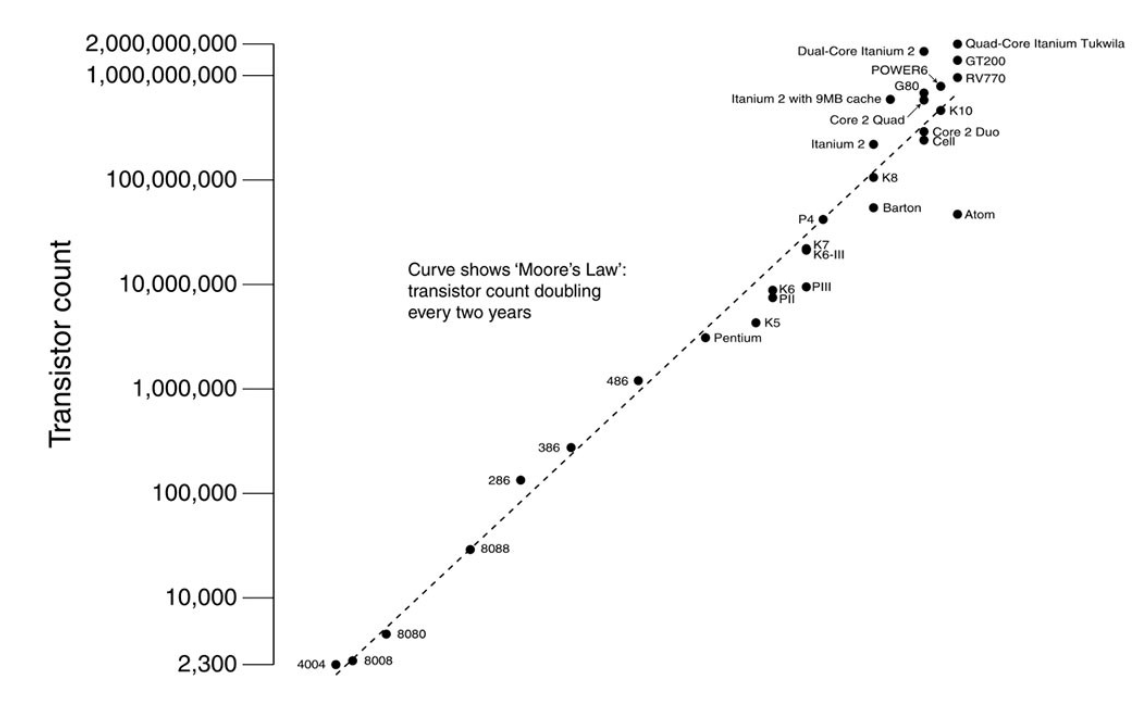
\includegraphics[scale=0.5]{imagenes/Herramientas/leymoore.png}
	\caption{La ley de Moore}
	\label{fig:La ley de Moore}
\end{figure}

La mayoría de los expertos, incluido el propio Moore esperan que esta apreciación se mantenga vigente hasta 2020-2025 donde dejará de cumplirse definitivamente . El estancamiento de la ley de Moore es la consecuencia de los límites físicos de la tecnología actual, en la que un número mayor de transistores para un mismo volumen se traduce en un mayor calor generado que no se va a poder disipar sin dañar el microcontrolador (Enfriar los transistores requiere más energía de la que pasa por los transistores).\newline 
 Este estancamiento de la tecnología de los microprocesadores, hará que no se pueda equiparar la potencia a la continua mejora de la velocidad de sus algoritmos; por lo que será necesario la búsqueda de nuevas tecnologías para que las empresas puedan seguir desarrollando sus productos.\newline

Aquí es donde entran en juego las FPGAs y el hecho de la importancia que están adquiriendo para las empresas su uso; ya que les permite multiplicar por un factor considerable la velocidad en sus circuitos. Las FPGAS se conocen desde los años 80, pero era una tecnología cerrada que muy pocos podían usar; además, las herramientas para manejarlas eran muy complejas. Todo cambió con la llegada de las FPGAS "libres", que ha propiciado que muchos aficionados creen herramientas para poder manejarlas de una manera más intuitiva y sencilla. \newline

\subsection{FPGAS libres}

El término \textit{libre} se refiere a los productos que se han diseñado específicamente para que sean totalmente accesibles para todos los usuarios, disponiendo de total libertad para utilizar, modificar y trabajar con estos productos. 
Las ventajas que permiten son enormes para el patrimonio tecnológico. Normalmente son mucho más fiables ya que hay un gran número de usuarios que trabajan para hacer que llegue a más gente. \newline

A las FPGAs les llegó su momento en mayo del 2015, en el panorama cambió con el Proyecto IceStorm creado por el ingeniero austríaco Clifford Wolf. \newline Wolf hizo ingeniería inversa de una de la FPGA ICE40 de Lattice para obtener toda la información de funcionamiento y poder crear herramientas libres que no dependieran de ningún fabricante. Esto permitió un gran desarrollo del sector ya que rápidamente se creó una gran comunidad.
La placa que usaremos para el proyecto será la Icezum Alhambra, pero existe una amplia variedad de placas con FPGAs libres.

\subsubsection{Icezum Alhambra II}

Tras un pequeño estudio del mercado de las FPGAs libres, la placa Icezum Alhambra II será la que utilicemos para este proyecto, ya que esta enfocada a la docencia. Tanto la primera versión como la revisión fueron diseñadas en Pinos del Valle(Granada) por Eladio Delgado. Sus dimensiones y apariencia es muy similar al de la placa Arduino UNO: el objetivo era que fuera compatible con la mayoría de Shields de Arduino, que son placas de circuitos modulares que le dan funcionalidades extras. Además, como hemos cometado anteriormente es una placa que está pensada para el aprendizaje, por lo que cuenta con bastantes añadidos como LEDs y pulsadores para que sea más fácil y cómodo su uso para pequeños proyectos.

\begin{figure}[H]
	\center
	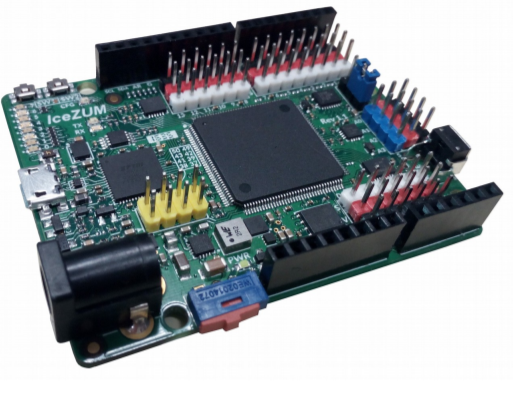
\includegraphics[scale=0.6]{imagenes/Herramientas/Icezum.png}
	\caption{Icezum Alhambra II}
	\label{fig:Icezum Alhambra II}
\end{figure}

Las características principales de la \textit{Icezum Alhambra II} son:

\begin{itemize}

	\item Placa de desarrollo con FPGA iCE40HX4K (Lattice) .
	\item Hardware abierto.
	\item Compatible con Icestudio.
	\item Se pueden reutilizar la mayoría de los shield disponibles en Arduino.
	\item Placa recomendada para proyectos robóticos.
	\item El dispositivo USB FTDI 2232H permite la programación de la FPGA y la interfaz UART la conexión a un PC.
	\item Interruptor electrónico de encendido/apagado.
	\item 8 LED de uso general (LED de usuario).
	\item 2 botones de propósito general.
	\item Memoria flash de 32 Mb.
	\item 20 pines de entrada / salida de 3.3V (tolera 5V).
	\item Todos los pines de E/S incluyen resistencias en serie de 200 ohmios para la activación directa de LED.
	\item Convertidor A/D de 4 canales y 12 bits.
	\item Pines de arranque en frío accesibles desde GPIO.
	\item Reguladores de conmutación para procesamiento de alta frecuencia a baja potencia de entrada.
	\item Oscilador MEMS de 12 MHZ.
	\item Botón de reinicio.
	\item Fuente de alimentación USB, dos conectores (hasta 4.8A).
\end{itemize}


\begin{figure}[H]
	\center
	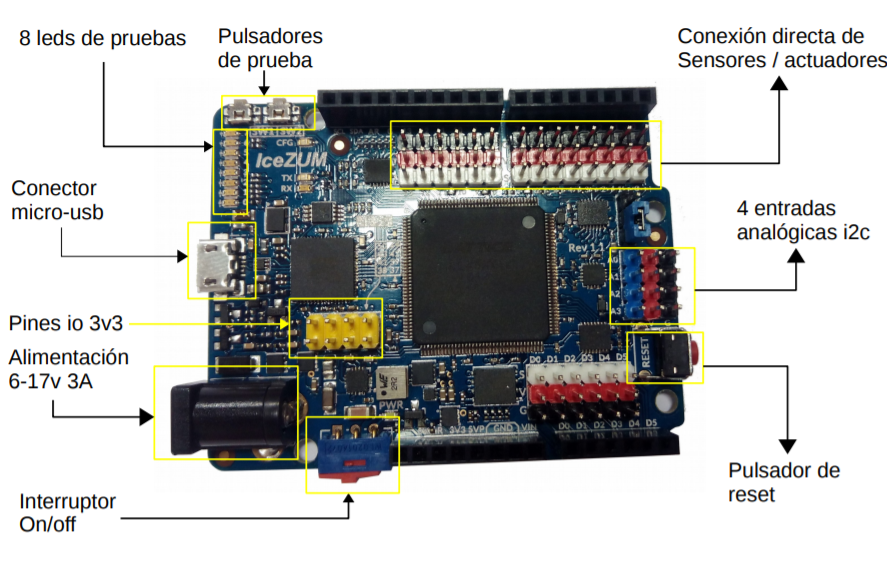
\includegraphics[scale=0.6]{imagenes/Herramientas/Icezum2.png}
	\caption{Icezum Alhambra II}
	\label{fig:Icezum Alhambra II}
\end{figure}

\newpage
\subsubsection{Icestudio}

Icestudio se trata de un editor visual para FPGAs libres, el cual está construido sobre el proyecto IceStorm usando Apio. Apio es una serie de herramientras multiplatarforma para FPGAS libres, con paquetes preconstruidos estáticos, herramientas de configuración de proyectos y una interfaz de comando fácil para verificar, sintetizar, simular y cargar diseños en Verilog. \newline

Icestudio surje de la necesidad de simplificar la ardua tarea que implica el aprendizaje de lenguajes HDL, haciéndolos más accesibles para todos.  Éste permite el diseño dor forma bastante sencilla para FPGAS mediante la creación de bloques con funcionalidades definidas. Se utiliza el lenguaje de descripción hardware Verilog para la creación de estos bloques, que se indica al usuario como puertas lógicas y biestables.  \newline

En la figura \ref{fig:Icestudio} se muestra la interfaz del programa. En la parte central es donde se colocan los bloques creados previamente, los cuales se relacionan para crear funcionalidades. También podremos seleccionar que puertos de estos bloques son entradas y cuales salidas; así como introducir bits como lo deseemos. En la parte superior se encuentran todas las herramientas disponibles para trabajar con Icestudio, para compilar el código una vez creado y cargarlo en la FPGA.

\vspace{5mm}

\begin{figure}[H]
	\center
	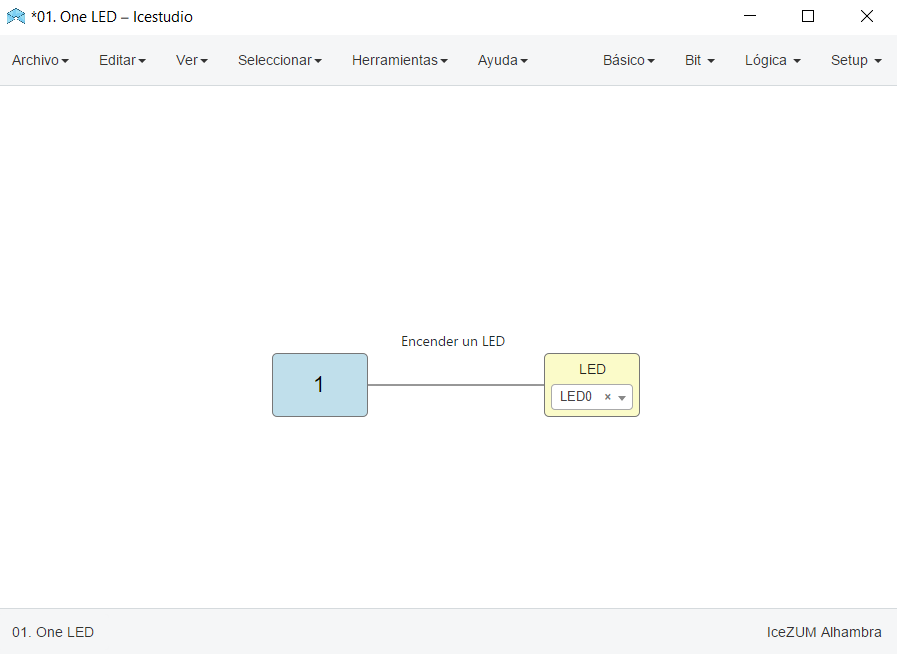
\includegraphics[scale=0.8]{imagenes/Herramientas/ice.png}
	\caption{Interfaz de Icestudio}
	\label{fig:Icestudio}
\end{figure}



